% Options for packages loaded elsewhere
% Options for packages loaded elsewhere
\PassOptionsToPackage{unicode}{hyperref}
\PassOptionsToPackage{hyphens}{url}
\PassOptionsToPackage{dvipsnames,svgnames,x11names}{xcolor}
%
\documentclass[
  spanish,
  11pt,
  letterpaper,
  DIV=11,
  numbers=noendperiod]{scrartcl}
\usepackage{xcolor}
\usepackage[left=3cm,right=3cm,top=3cm,bottom=3cm]{geometry}
\usepackage{amsmath,amssymb}
\setcounter{secnumdepth}{-\maxdimen} % remove section numbering
\usepackage{iftex}
\ifPDFTeX
  \usepackage[T1]{fontenc}
  \usepackage[utf8]{inputenc}
  \usepackage{textcomp} % provide euro and other symbols
\else % if luatex or xetex
  \usepackage{unicode-math} % this also loads fontspec
  \defaultfontfeatures{Scale=MatchLowercase}
  \defaultfontfeatures[\rmfamily]{Ligatures=TeX,Scale=1}
\fi
\usepackage{lmodern}
\ifPDFTeX\else
  % xetex/luatex font selection
\fi
% Use upquote if available, for straight quotes in verbatim environments
\IfFileExists{upquote.sty}{\usepackage{upquote}}{}
\IfFileExists{microtype.sty}{% use microtype if available
  \usepackage[]{microtype}
  \UseMicrotypeSet[protrusion]{basicmath} % disable protrusion for tt fonts
}{}
\makeatletter
\@ifundefined{KOMAClassName}{% if non-KOMA class
  \IfFileExists{parskip.sty}{%
    \usepackage{parskip}
  }{% else
    \setlength{\parindent}{0pt}
    \setlength{\parskip}{6pt plus 2pt minus 1pt}}
}{% if KOMA class
  \KOMAoptions{parskip=half}}
\makeatother
% Make \paragraph and \subparagraph free-standing
\makeatletter
\ifx\paragraph\undefined\else
  \let\oldparagraph\paragraph
  \renewcommand{\paragraph}{
    \@ifstar
      \xxxParagraphStar
      \xxxParagraphNoStar
  }
  \newcommand{\xxxParagraphStar}[1]{\oldparagraph*{#1}\mbox{}}
  \newcommand{\xxxParagraphNoStar}[1]{\oldparagraph{#1}\mbox{}}
\fi
\ifx\subparagraph\undefined\else
  \let\oldsubparagraph\subparagraph
  \renewcommand{\subparagraph}{
    \@ifstar
      \xxxSubParagraphStar
      \xxxSubParagraphNoStar
  }
  \newcommand{\xxxSubParagraphStar}[1]{\oldsubparagraph*{#1}\mbox{}}
  \newcommand{\xxxSubParagraphNoStar}[1]{\oldsubparagraph{#1}\mbox{}}
\fi
\makeatother


\usepackage{longtable,booktabs,array}
\newcounter{none} % for unnumbered tables
\usepackage{calc} % for calculating minipage widths
% Correct order of tables after \paragraph or \subparagraph
\usepackage{etoolbox}
\makeatletter
\patchcmd\longtable{\par}{\if@noskipsec\mbox{}\fi\par}{}{}
\makeatother
% Allow footnotes in longtable head/foot
\IfFileExists{footnotehyper.sty}{\usepackage{footnotehyper}}{\usepackage{footnote}}
\makesavenoteenv{longtable}
\usepackage{graphicx}
\makeatletter
\newsavebox\pandoc@box
\newcommand*\pandocbounded[1]{% scales image to fit in text height/width
  \sbox\pandoc@box{#1}%
  \Gscale@div\@tempa{\textheight}{\dimexpr\ht\pandoc@box+\dp\pandoc@box\relax}%
  \Gscale@div\@tempb{\linewidth}{\wd\pandoc@box}%
  \ifdim\@tempb\p@<\@tempa\p@\let\@tempa\@tempb\fi% select the smaller of both
  \ifdim\@tempa\p@<\p@\scalebox{\@tempa}{\usebox\pandoc@box}%
  \else\usebox{\pandoc@box}%
  \fi%
}
% Set default figure placement to htbp
\def\fps@figure{htbp}
\makeatother



\ifLuaTeX
\usepackage[bidi=basic,shorthands=off]{babel}
\else
\usepackage[bidi=default,shorthands=off]{babel}
\fi
\ifLuaTeX
  \usepackage{selnolig} % disable illegal ligatures
\fi


\setlength{\emergencystretch}{3em} % prevent overfull lines

\providecommand{\tightlist}{%
  \setlength{\itemsep}{0pt}\setlength{\parskip}{0pt}}



 


\usepackage{booktabs}
\usepackage{longtable}
\usepackage{array}
\usepackage{multirow}
\usepackage{wrapfig}
\usepackage{float}
\usepackage{colortbl}
\usepackage{pdflscape}
\usepackage{tabularx}
\usepackage{xltabular}
\usepackage{threeparttable}
\usepackage{threeparttablex}
\usepackage[normalem]{ulem}
\usepackage{makecell}
\usepackage{xcolor}
\KOMAoption{captions}{tableheading}
\usepackage{caption}
\captionsetup[table]{position=bottom,labelformat=default,labelsep=colon,name=Tabla}
\captionsetup[figure]{labelformat=default,labelsep=colon,name=Figura}
\usepackage{float}
\floatplacement{figure}{H}
\makeatletter
\@ifpackageloaded{caption}{}{\usepackage{caption}}
\AtBeginDocument{%
\ifdefined\contentsname
  \renewcommand*\contentsname{Tabla de contenidos}
\else
  \newcommand\contentsname{Tabla de contenidos}
\fi
\ifdefined\listfigurename
  \renewcommand*\listfigurename{Listado de Figuras}
\else
  \newcommand\listfigurename{Listado de Figuras}
\fi
\ifdefined\listtablename
  \renewcommand*\listtablename{Listado de Tablas}
\else
  \newcommand\listtablename{Listado de Tablas}
\fi
\ifdefined\figurename
  \renewcommand*\figurename{Figura}
\else
  \newcommand\figurename{Figura}
\fi
\ifdefined\tablename
  \renewcommand*\tablename{Tabla}
\else
  \newcommand\tablename{Tabla}
\fi
}
\@ifpackageloaded{float}{}{\usepackage{float}}
\floatstyle{ruled}
\@ifundefined{c@chapter}{\newfloat{codelisting}{h}{lop}}{\newfloat{codelisting}{h}{lop}[chapter]}
\floatname{codelisting}{Listado}
\newcommand*\listoflistings{\listof{codelisting}{Listado de Listados}}
\makeatother
\makeatletter
\makeatother
\makeatletter
\@ifpackageloaded{caption}{}{\usepackage{caption}}
\@ifpackageloaded{subcaption}{}{\usepackage{subcaption}}
\makeatother
\usepackage{bookmark}
\IfFileExists{xurl.sty}{\usepackage{xurl}}{} % add URL line breaks if available
\urlstyle{same}
\hypersetup{
  pdflang={es-ES},
  colorlinks=true,
  linkcolor={blue},
  filecolor={Maroon},
  citecolor={Blue},
  urlcolor={Blue},
  pdfcreator={LaTeX via pandoc}}


\author{}
\date{}
\begin{document}


\begin{titlepage}
  \centering

  \includegraphics[width=0.7\textwidth]{logo_facultad.png}\par

  \vspace{3cm}

  {\scshape\Huge Trabajo Práctico de Series de Tiempo \par}

  \vspace{1.5cm}

  {\itshape\LARGE Análisis de muertes por Accidentes Cerebrovasculares (ACV) en Estados Unidos \par}

  \vfill

  {\Large Alumna: Cañizares, María Inés \par}

  \vspace{0.5cm}

  {\Large Licenciatura en Estadística \par}

  \vspace{1cm}

  {\large Año 2026 \par}

\end{titlepage}

\section{Introducción}\label{introducciuxf3n}

El Accidente Cerebrovascular (ACV), conocido popularmente como ``derrame
cerebral'' o ``ataque cerebral'', es una afección médica que ocurre
cuando se interrumpe el flujo de sangre hacia una parte del cerebro, ya
sea porque un vaso sanguíneo se obstruye o porque se rompe. Esta
interrupción hace que las células cerebrales de la zona afectada dejen
de recibir oxígeno y nutrientes, lo que puede provocar daños permanentes
en cuestión de minutos.

El ACV es uno de los principales problemas de salud pública a nivel
mundial. Es una de las principales causas de muerte y, entre quienes
sobreviven, una de las principales causas de discapacidad a largo plazo,
ya que puede dejar secuelas como parálisis, dificultades para hablar o
problemas cognitivos. Además, es una enfermedad estrechamente
relacionada con factores que varían a lo largo del año, como la presión
arterial y la temperatura ambiente, lo que la convierte en un fenómeno
interesante para analizar desde una perspectiva temporal: ¿la cantidad
de muertes por esta causa se mantiene estable a lo largo de los años, o
cambia? ¿Existen ciertas épocas del año donde el riesgo es mayor?

Entender cómo evoluciona la mortalidad por ACV a través del tiempo es
relevante no solo desde el punto de vista médico, sino también para la
planificación de recursos sanitarios: si se pudiera anticipar en qué
meses o períodos aumenta el riesgo, los sistemas de salud podrían
prepararse mejor (por ejemplo, reforzando personal o insumos en los
meses de mayor demanda).

Por este motivo, en este trabajo se analiza la evolución mensual de la
cantidad de muertes por ACV en Estados Unidos entre los años 1999 y
2019, utilizando datos públicos provenientes de CDC WONDER, una base de
datos oficial del gobierno estadounidense que recopila estadísticas
vitales del país. El objetivo es describir el comportamiento de esta
serie a lo largo del tiempo e identificar si existen patrones
recurrentes, como tendencias de largo plazo o variaciones estacionales
asociadas a las distintas épocas del año.

\section{Análisis descriptivo de la serie
temporal}\label{anuxe1lisis-descriptivo-de-la-serie-temporal}

Se presenta la serie temporal de las muertes por ACV mensual en Estados
Unidos durante el período 1999--2018. El gráfico permite visualizar de
manera global cómo se ha comportado la variable en el tiempo.

\begin{figure}

\centering{

\pandocbounded{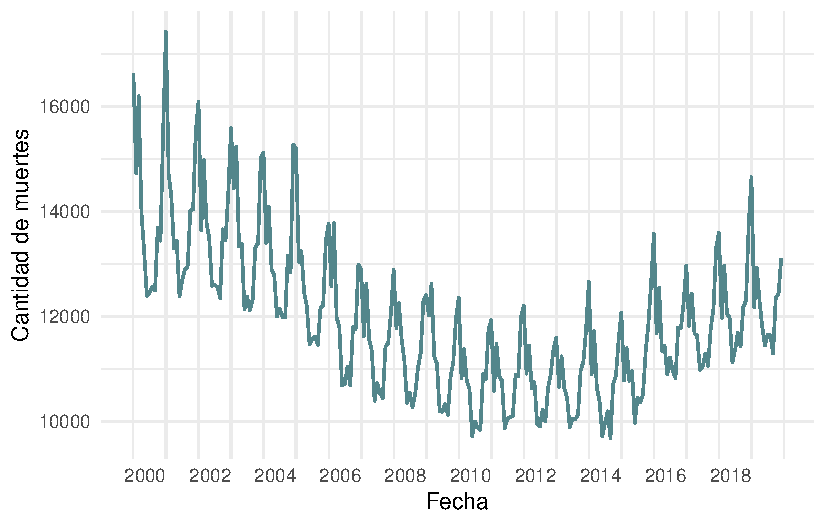
\includegraphics[keepaspectratio]{TP-MInesCañizares_files/figure-pdf/fig-serie-1.pdf}}

}

\caption{\label{fig-serie}Evolución de las muertes mensuales por ACV en
Estados Unidos (1999--2018)}

\end{figure}%

El análisis de la serie muestra que se trata de una variable con
periodicidad mensual, con 12 observaciones por año. En cuanto a la
tendencia, no se observa un comportamiento uniforme a lo largo de todo
el período: entre 1999 y 2010 se registra un descenso sostenido en la
cantidad de muertes, mientras que a partir de 2011 la serie comienza a
mostrar una recuperación progresiva, con un crecimiento que se mantiene
hasta el final del período en 2018. Este patrón refleja un cambio de
dirección en la tendencia, describiendo una forma de ``U'' a lo largo de
los veinte años analizados, lo que indica que la serie no es
estacionaria en media.

Respecto a la estacionalidad, se observa un comportamiento recurrente
año tras año, caracterizado por valores máximos en los meses de invierno
(diciembre, enero y febrero) y valores mínimos en los meses de verano
(junio a septiembre). No se detectaron valores faltantes en el período
estudiado.

Con el fin de profundizar en el análisis de la tendencia y la
variabilidad de la serie, se construyó un gráfico de boxplots anuales
(Figura 2), que permite visualizar la distribución de los datos mes a
mes agrupados por año.

\begin{figure}

\centering{

\pandocbounded{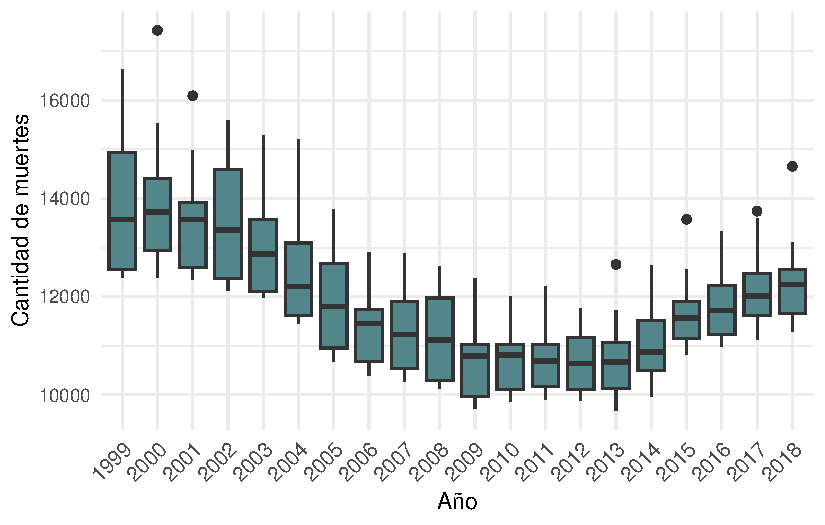
\includegraphics[keepaspectratio]{TP-MInesCañizares_files/figure-pdf/fig-boxplot-1.pdf}}

}

\caption{\label{fig-boxplot}Distribución anual de las muertes por ACV en
Estados Unidos (1999--2018)}

\end{figure}%

Las medianas anuales confirman el mismo patrón en forma de ``U''
descrito anteriormente: descienden desde 1999 hasta aproximadamente
2010-2011, para luego aumentar de manera sostenida hasta 2018.

En cuanto a la dispersión, se observa que la amplitud de las cajas
(rango intercuartílico) no se mantiene constante a lo largo del período:
es mayor en los primeros años de la serie (1999-2003) y en los últimos
(2016-2018), mientras que se reduce notablemente durante los años
centrales (2008-2013). Esta variación en la dispersión acompaña al nivel
general de la serie, lo que sugiere que la variancia no es estable en el
tiempo, es decir, se evidencia heterocedasticidad.

Asimismo, se identifican algunos valores atípicos (outliers) en
determinados años, correspondientes principalmente a meses de invierno
con picos de mortalidad inusualmente altos respecto al resto de las
observaciones de ese mismo año.

Para analizar con mayor detalle el comportamiento estacional de la
serie, se elaboró un gráfico estacional (Figura 3), en el cual se
superponen las observaciones de cada año, ordenadas por mes, con el fin
de comparar la forma del patrón estacional entre los distintos años.

\begin{figure}

\centering{

\pandocbounded{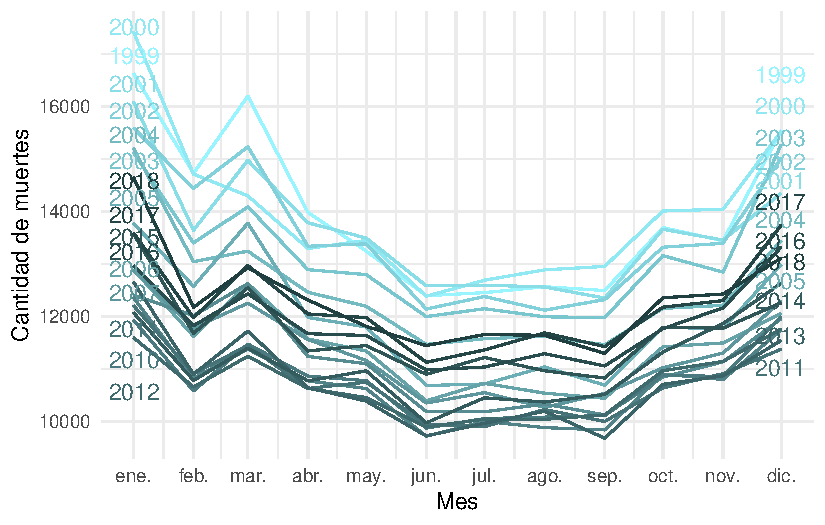
\includegraphics[keepaspectratio]{TP-MInesCañizares_files/figure-pdf/fig-season-1.pdf}}

}

\caption{\label{fig-season}Gráfico estacional de las muertes por ACV en
Estados Unidos (1999--2018)}

\end{figure}%

Se observa que la forma del ciclo estacional se mantiene notablemente
estable a lo largo de todo el período: en todos los años, los valores
más altos se concentran en los meses de diciembre y enero, mientras que
los valores más bajos se registran entre junio y septiembre. Lo que
varía entre los distintos años no es la forma de la curva, sino su nivel
general, lo cual es consistente con la tendencia en forma de ``U''
identificada previamente: las curvas correspondientes a los primeros
años (1999-2003) y a los últimos (2016-2018) se ubican en niveles más
altos, mientras que las curvas de los años centrales (2008-2013) se
ubican en niveles más bajos. En síntesis, el gráfico estacional confirma
la presencia de un patrón estacional anual marcado y persistente en el
tiempo, lo que refuerza la evidencia de no estacionariedad de la serie
observada en los análisis anteriores.

Con el objetivo de aislar el efecto de cada mes en particular a lo largo
de toda la serie, se construyó un gráfico de subseries estacionales,
donde cada panel representa un mes del año y la línea horizontal indica
el promedio histórico de ese mes para todo el período analizado.

\begin{figure}

\centering{

\pandocbounded{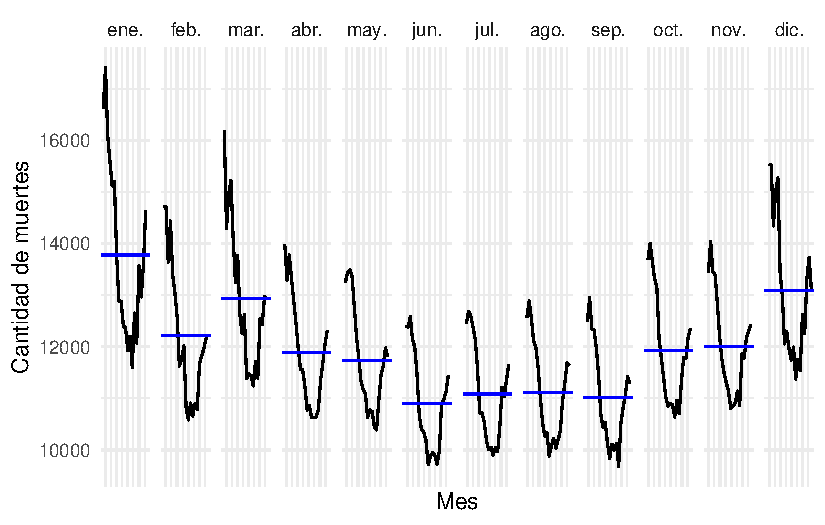
\includegraphics[keepaspectratio]{TP-MInesCañizares_files/figure-pdf/fig-subseries-1.pdf}}

}

\caption{\label{fig-subseries}Gráfico de subseries estacionales de las
muertes por ACV en Estados Unidos (1999--2018)}

\end{figure}%

La Figura 4 confirma lo observado en las figuras anteriores: los meses
de diciembre y enero presentan los promedios más altos de mortalidad,
mientras que los meses de junio a septiembre muestran los promedios más
bajos, evidenciando nuevamente el patrón estacional de tipo
invierno-verano. Asimismo, dentro de cada panel se puede apreciar que la
evolución temporal del mes correspondiente también sigue la forma de
``U'' identificada en la tendencia general de la serie, lo que indica
que este comportamiento no solo se da en el nivel agregado, sino que se
repite de manera consistente mes a mes. En conjunto, este gráfico
refuerza la evidencia de un componente estacional fuerte y estable en el
tiempo, que convive con una tendencia no constante a lo largo del
período estudiado.

Finalmente, para contar con una confirmación estadística de las
características observadas en los gráficos anteriores, se calculó la
función de autocorrelación muestral, considerando hasta 36 rezagos.

\begin{figure}

\centering{

\pandocbounded{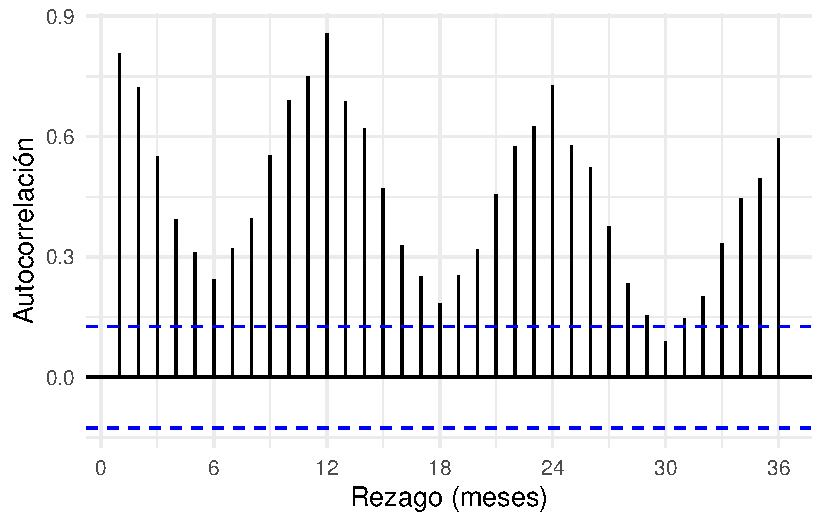
\includegraphics[keepaspectratio]{TP-MInesCañizares_files/figure-pdf/fig-acf-1.pdf}}

}

\caption{\label{fig-acf}Función de autocorrelación de las muertes por
ACV}

\end{figure}%

En la Figura 5 se observa un pico de autocorrelación particularmente
alto en el rezago 12, que vuelve a repetirse con menor intensidad en los
rezagos 24 y 36, lo cual constituye evidencia formal de la
estacionalidad anual detectada previamente de manera gráfica. Asimismo,
se observa que las autocorrelaciones no decaen rápidamente hacia cero a
medida que aumenta el rezago, sino que lo hacen de forma lenta y
sostenida, manteniéndose por encima de la banda de significancia en la
gran mayoría de los rezagos analizados. Este comportamiento es
característico de series no estacionarias, ya que refleja la presencia
de una dependencia de largo plazo asociada tanto a la tendencia como a
la estacionalidad presentes en la serie. En síntesis, el correlograma
confirma de manera formal lo observado en el análisis gráfico previo,
evidenciando que la serie no es estacionaria ni en media ni en varianza.

Complementando el análisis de la función de autocorrelación, se calculó
también la función de autocorrelación parcial, que permite identificar
la correlación directa entre una observación y su rezago, eliminando el
efecto de los rezagos intermedios.

\begin{figure}

\centering{

\pandocbounded{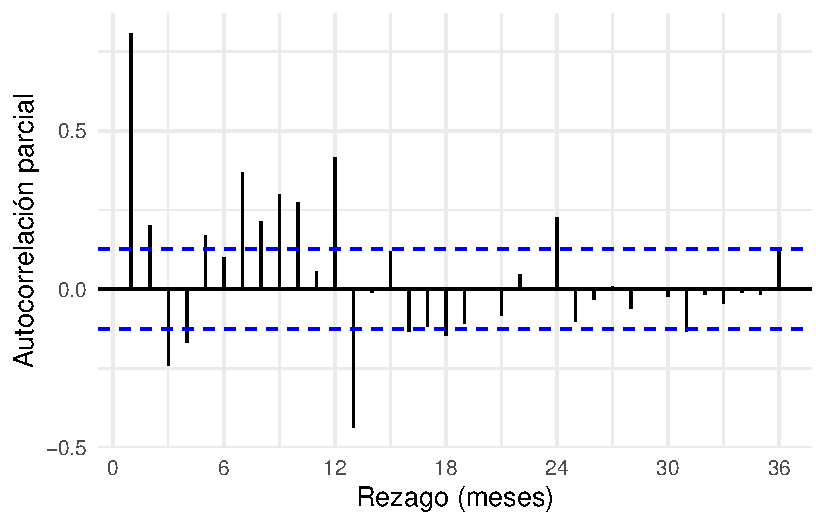
\includegraphics[keepaspectratio]{TP-MInesCañizares_files/figure-pdf/fig-pacf-1.pdf}}

}

\caption{\label{fig-pacf}Función de Autocorrelación Parcial de las
muertes por ACV}

\end{figure}%

La Figura~\ref{fig-pacf} muestra un primer coeficiente muy elevado en el
rezago 1 (cercano a 0,8), seguido de varios coeficientes significativos
de menor magnitud entre los rezagos 2 y 10, con signos alternantes. Se
destaca además un coeficiente marcadamente negativo en el rezago 12
(cercano a -0,4), que resulta notablemente mayor en valor absoluto que
el resto de los coeficientes a partir del rezago 13, los cuales se
ubican mayormente dentro de la banda de significancia o apenas por fuera
de ella, salvo un pico aislado cercano al rezago 24. Este comportamiento
sugiere que, además de la dependencia de corto plazo reflejada en los
primeros rezagos, persiste cierta estructura asociada al componente
estacional de la serie, evidenciada por el coeficiente significativo en
el rezago 12. En conjunto, el correlograma parcial refuerza la idea de
que la serie presenta una estructura de dependencia compleja,
consistente con la presencia simultánea de componentes de corto plazo y
de estacionalidad, lo que confirma nuevamente que la serie no es
estacionaria en su forma original.

\section{Especificación del modelo}\label{especificaciuxf3n-del-modelo}

En primer lugar, con el objetivo de evaluar si la variabilidad cambia
con el nivel de la serie, se analizó la relación entre la media anual y
el desvío estándar anual. Esta relación permite observar si existe una
tendencia creciente entre ambos valores: cuando las observaciones de
mayor nivel también muestran una mayor dispersión, suele ser indicio de
varianza no constante y, por lo tanto, puede justificar la aplicación de
una transformación Box--Cox para estabilizarla.

\begin{figure}

\centering{

\pandocbounded{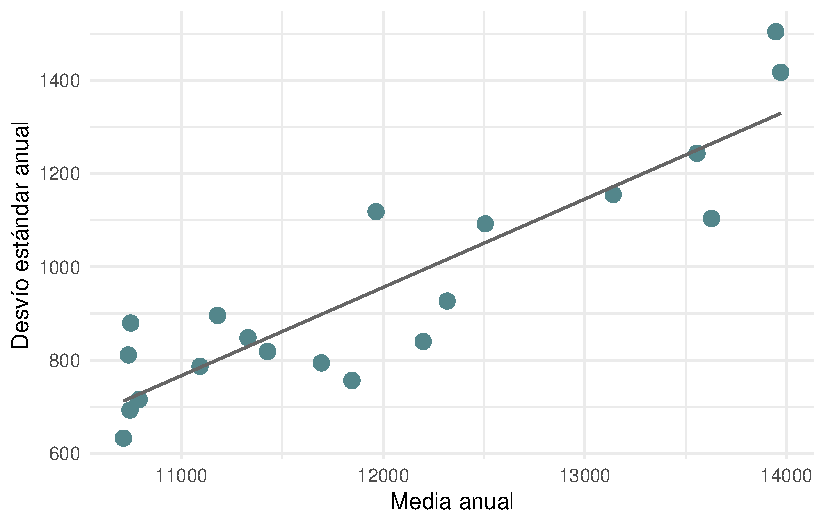
\includegraphics[keepaspectratio]{TP-MInesCañizares_files/figure-pdf/fig-media-desvio-1.pdf}}

}

\caption{\label{fig-media-desvio}Relación entre media y desvío estándar
anual}

\end{figure}%

La Figura~\ref{fig-media-desvio} muestra una relación creciente, lo que
indica que la variancia depende del nivel de la serie.

\begin{figure}[H]

{\centering \pandocbounded{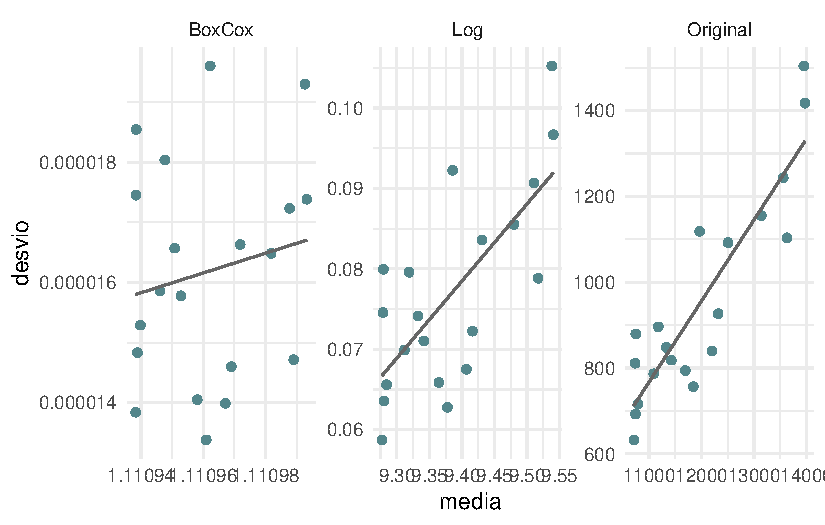
\includegraphics[keepaspectratio]{TP-MInesCañizares_files/figure-pdf/unnamed-chunk-6-1.pdf}}

}

\caption{Transformaciones de variancia}

\end{figure}%

La transformación logarítmica reduce, pero no elimina, esta dependencia.
En cambio, la transformación de Box-Cox con \(\lambda ≈ −0{,}9\)
(estimado por el método de Guerrero) deja el desvío aproximadamente
constante respecto de la media, por lo que se adopta para el resto del
análisis.

Una vez evaluada la necesidad de estabilizar la variancia, el siguiente
paso consiste en lograr que la serie sea estacionaria en media. Para
ello se emplea la diferenciación, que elimina patrones sistemáticos de
la serie: la diferenciación regular, \((1-B)^d\), elimina tendencias de
largo plazo, y la diferenciación estacional, \((1-B^{12})^D\), elimina
las fluctuaciones que se repiten de forma regular cada año.

Para determinar los órdenes \(d\) y \(D\) se emplearon pruebas de raíz
unitaria (basadas en el estadístico KPSS), complementadas con el
análisis gráfico de la serie y de sus funciones de autocorrelación. Dada
la marcada estacionalidad anual, se aplicó primero la diferencia
estacional, siguiendo la recomendación de Hyndman y Athanasopoulos.

\begin{figure}

\centering{

\pandocbounded{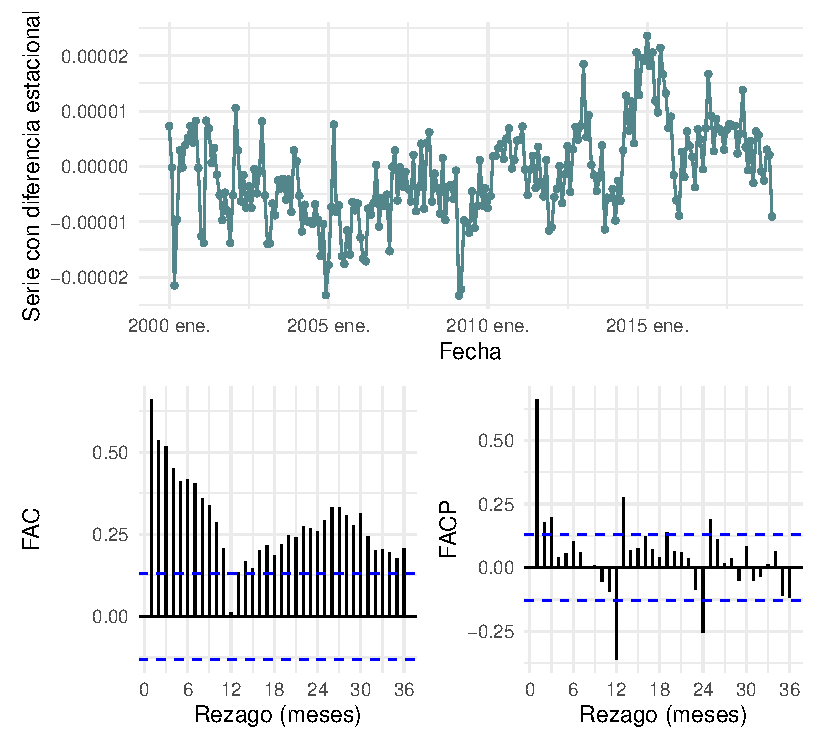
\includegraphics[keepaspectratio]{TP-MInesCañizares_files/figure-pdf/fig-dif-estacional-1.pdf}}

}

\caption{\label{fig-dif-estacional}Serie transformada con una diferencia
estacional, con su FAC y FACP}

\end{figure}%

La prueba indicó que se requiere una diferencia estacional. Sin embargo,
al observar la serie con diferencia estacional
(Figura~\ref{fig-dif-estacional}), se ve que su nivel se desplaza a lo
largo del tiempo, con un tramo de valores altos entre 2013 y 2016, y que
su función de autocorrelación decae lentamente, con valores positivos y
significativos en casi todos los rezagos. Esto indica que persiste una
tendencia. Coincidentemente, la prueba para diferencias regulares
aplicada sobre esta serie indicó una diferencia adicional.

\begin{figure}

\centering{

\pandocbounded{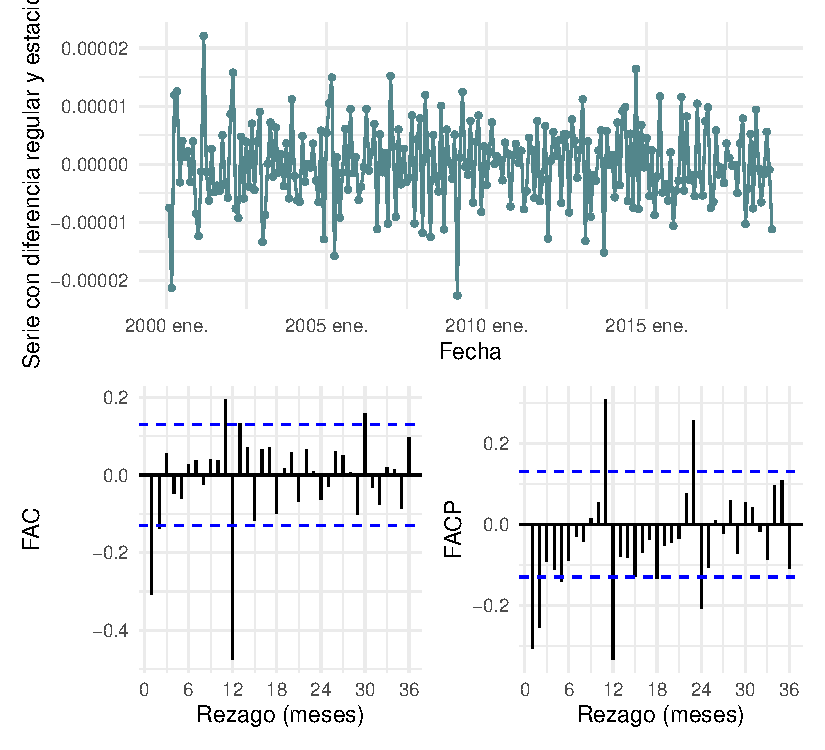
\includegraphics[keepaspectratio]{TP-MInesCañizares_files/figure-pdf/fig-dif-ambas-1.pdf}}

}

\caption{\label{fig-dif-ambas}Serie transformada con una diferencia
regular y una estacional, con su FAC y FACP}

\end{figure}%

Al aplicar ambas diferencias (Figura~\ref{fig-dif-ambas}), la serie
oscila alrededor de cero con variabilidad aproximadamente constante y
sin tendencia aparente. Además, la autocorrelación en el rezago 1 es
cercana a \(-0{,}3\), lejos del valor de \(-0{,}5\) a partir del cual
suele sospecharse sobrediferenciación. Se adopta entonces \(d = 1\) y
\(D = 1\).

\subsection{Identificación de modelos
candidatos}\label{identificaciuxf3n-de-modelos-candidatos}

A partir de la FAC y la FACP de la serie diferenciada
(Figura~\ref{fig-dif-ambas}):

\begin{itemize}
\tightlist
\item
  En la FAC hay un pico negativo en el rezago 1 y otro más marcado en el
  rezago 12, con valores pequeños alrededor de los rezagos 11 y 13. Es
  un patrón característico de un término de promedios móviles no
  estacional de orden 1 y de uno estacional de orden 1.
\item
  En la FACP los rezagos 1 y 2 son negativos y significativos, y en la
  parte estacional los rezagos 12 y 24 son negativos con magnitud
  decreciente. Esto es consistente con la parte de promedios móviles
  estacional y sugiere que podría hacer falta un segundo término de
  promedios móviles no estacional.
\end{itemize}

Se proponen entonces tres modelos candidatos,
\(\text{SARIMA}(p,d,q)(P,D,Q)_{12}\): (1) \((0,1,1)(0,1,1)\), (2)
\((0,1,2)(0,1,1)\) y (3) \((2,1,0)(2,1,0)\), este último como
alternativa puramente autorregresiva sugerida por la FACP. Se incluye
además, como referencia, el modelo seleccionado por el algoritmo
automático de búsqueda.

\section{Ajuste y diagnóstico}\label{ajuste-y-diagnuxf3stico}

Los modelos se estimaron por máxima verosimilitud sobre la serie
transformada. Como todos comparten la misma transformación y los mismos
órdenes de diferenciación, pueden compararse mediante AICc y BIC
(Tabla~\ref{tbl-aicc}).

{

\begin{longtable}[]{@{}ccc@{}}

\caption{\label{tbl-aicc}Comparación de los modelos candidatos}

\tabularnewline

\toprule\noalign{}
Modelo & AICc & BIC \\
\midrule\noalign{}
\endhead
\bottomrule\noalign{}
\endlastfoot
ARIMA(0,1,2)(0,1,1){[}12{]} & -4874.32 & -4860.80 \\
ARIMA(0,1,1)(0,1,1){[}12{]} & -4870.79 & -4860.62 \\
Automático: ARIMA(0,1,1)(2,1,2){[}12{]} & -4868.60 & -4848.43 \\
ARIMA(2,1,0)(2,1,0){[}12{]} & -4853.04 & -4836.19 \\

\end{longtable}

}

El modelo \(\text{SARIMA}(0,1,2)(0,1,1)_{12}\) presenta los menores
valores de AICc y BIC. El modelo automático, que resultó ser un
\(\text{SARIMA}(0,1,1)(2,1,2)_{12}\), es más complejo y casi todos sus
coeficientes estacionales no son significativos, lo que sugiere
sobreparametrización. El modelo autorregresivo es el de peor ajuste.

Se realiza el ajuste para el modelo \(\text{ARIMA}(0,1,2)(0,1,1)_{12}\)
sobre la serie transformada \(Z_t\):

\[(1-B)(1-B^{12})Z_t = (1-\theta_1 B-\theta_2 B^2)(1-\Theta_1 B^{12})\,a_t,\]

donde \(Z_t\) es la serie transformada mediante Box-Cox con
\(\hat{\lambda} = -0{,}90\) y \(a_t\) es ruido blanco. De esta forma, el
modelo estimado queda:

\[(1-B)(1-B^{12})Z_t = (1-0{,}4580B-0{,}1598B^2)(1-0{,}7814B^{12})\,a_t.\]

{

\begin{longtable}[]{@{}
  >{\centering\arraybackslash}p{(\linewidth - 8\tabcolsep) * \real{0.1507}}
  >{\centering\arraybackslash}p{(\linewidth - 8\tabcolsep) * \real{0.1644}}
  >{\centering\arraybackslash}p{(\linewidth - 8\tabcolsep) * \real{0.2192}}
  >{\centering\arraybackslash}p{(\linewidth - 8\tabcolsep) * \real{0.2329}}
  >{\centering\arraybackslash}p{(\linewidth - 8\tabcolsep) * \real{0.2329}}@{}}

\caption{\label{tbl-coef-m2}Coeficientes estimados del modelo
SARIMA(0,1,2)(0,1,1){[}12{]}}

\tabularnewline

\toprule\noalign{}
\begin{minipage}[b]{\linewidth}\centering
Parámetro
\end{minipage} & \begin{minipage}[b]{\linewidth}\centering
Estimación
\end{minipage} & \begin{minipage}[b]{\linewidth}\centering
Error estándar
\end{minipage} & \begin{minipage}[b]{\linewidth}\centering
IC 95\% inferior
\end{minipage} & \begin{minipage}[b]{\linewidth}\centering
IC 95\% superior
\end{minipage} \\
\midrule\noalign{}
\endhead
\bottomrule\noalign{}
\endlastfoot
ma1 & -0.4580 & 0.0686 & -0.5925 & -0.3235 \\
ma2 & -0.1598 & 0.0663 & -0.2898 & -0.0298 \\
sma1 & -0.7814 & 0.0561 & -0.8914 & -0.6714 \\

\end{longtable}

}

Los tres coeficientes resultan significativos, ya que sus intervalos de
confianza del 95\% no contienen al cero (Tabla Tabla~\ref{tbl-coef-m2}).
Además, el coeficiente estacional (\(-0{,}78\)) se encuentra alejado de
\(-1\), por lo que el modelo es invertible.

Para el diagnóstico de los residuos se excluyeron las primeras 13
observaciones, cuyos residuos dependen de las condiciones iniciales de
la diferenciación.

Se procede entonces con el análisis de los residuos para este primer
modelo, iniciando con el Test de Portmanteau para verificar si la
hipótesis de que los mismos son ruido blanco se cumple:

{

\begin{longtable}[]{@{}cccc@{}}

\caption{\label{tbl-port-m2}Test de Portmanteau de los residuos del
modelo SARIMA(0,1,2)(0,1,1){[}12{]}}

\tabularnewline

\toprule\noalign{}
Rezago & Estadística & gl & p-value \\
\midrule\noalign{}
\endhead
\bottomrule\noalign{}
\endlastfoot
6 & 3.654 & 3 & 0.301 \\
12 & 15.131 & 9 & 0.087 \\
18 & 17.551 & 15 & 0.287 \\
24 & 24.919 & 21 & 0.251 \\

\end{longtable}

}

Los valores del test muestran que ningún p-value es significativo para
ninguno de los rezagos evaluados (todos mayores a 0.05), por lo que los
residuos se comportan como ruido blanco y no presentan autocorrelación
significativa.

\begin{figure}

\centering{

\pandocbounded{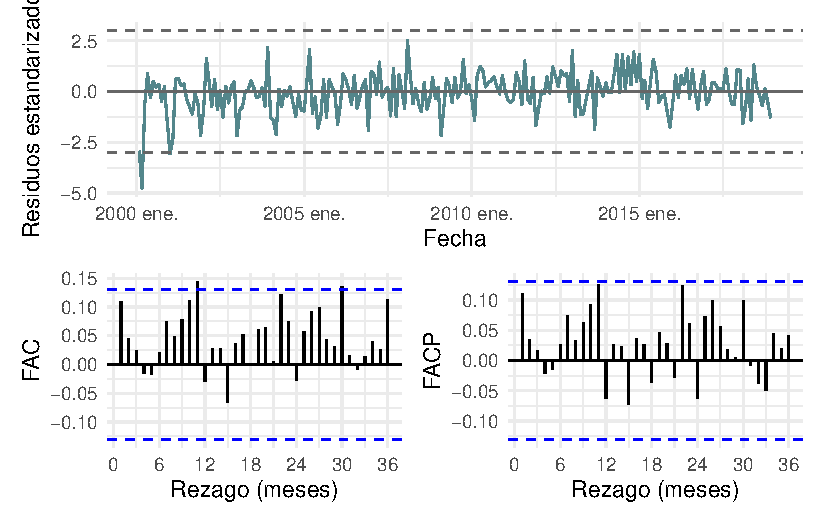
\includegraphics[keepaspectratio]{TP-MInesCañizares_files/figure-pdf/fig-res-m2-1.pdf}}

}

\caption{\label{fig-res-m2}Residuos estandarizados del modelo
ARIMA(0,1,2)(0,1,1){[}12{]}, con su FAC y FACP}

\end{figure}%

Los residuos estandarizados (Figura Figura~\ref{fig-res-m2}) oscilan
alrededor de cero con variabilidad aproximadamente constante. Se
identifica una observación al inicio de la serie por fuera del intervalo
\((-3, 3)\). La FAC y la FACP de los residuos se mantienen mayormente
dentro de las bandas de significancia, con un único rezago (el 12)
apenas por fuera en la FAC, lo cual es compatible con el azar al evaluar
36 rezagos y con el resultado del test de Portmanteau.

\begin{figure}

\centering{

\pandocbounded{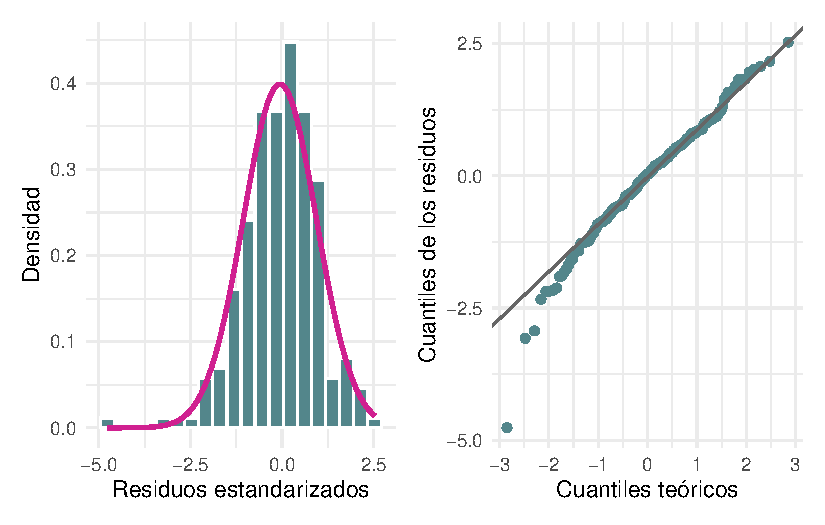
\includegraphics[keepaspectratio]{TP-MInesCañizares_files/figure-pdf/fig-norm-m2-1.pdf}}

}

\caption{\label{fig-norm-m2}Histograma y QQ-plot de los residuos
estandarizados del modelo ARIMA(0,1,2)(0,1,1){[}12{]}}

\end{figure}%

El histograma y el QQ-plot (Figura Figura~\ref{fig-norm-m2}) muestran
una distribución aproximadamente normal, con una cola izquierda algo más
pesada debida a los valores extremos mencionados. Además, se realizó el
test de Shapiro-Wilk, en donde se rechaza la hipótesis de normalidad de
los residuos (p-value = 0,0006). Este apartamiento se concentra en la
cola izquierda y se debe principalmente a dos observaciones atípicas,
correspondientes a marzo de 2000 y enero de 2001, cuyos residuos
estandarizados superan en valor absoluto el valor 3. Dado que el test de
Portmanteau no detecta autocorrelación remanente, la falta de normalidad
no afecta los pronósticos puntuales, pero sí podría afectar la exactitud
de los intervalos de pronóstico, que se construyen bajo el supuesto de
normalidad.

Se realiza el ajuste para el modelo \(\text{SARIMA}(0,1,1)(0,1,1)_{12}\)
sobre la serie transformada \(Z_t\):

\[(1-B)(1-B^{12})Z_t = (1-\theta_1 B)(1-\Theta_1 B^{12})\,a_t,\]

donde \(Z_t\) es la serie transformada mediante Box-Cox con
\(\hat{\lambda} = -0{,}90\) y \(a_t\) es ruido blanco. De esta forma, el
modelo estimado queda:

\[(1-B)(1-B^{12})Z_t = (1-0{,}5526B)(1-0{,}7872B^{12})\,a_t.\]

Se presenta una tabla con los valores de los coeficientes estimados,
acompañados de un IC para probar su significación.

{

\begin{longtable}[]{@{}
  >{\centering\arraybackslash}p{(\linewidth - 8\tabcolsep) * \real{0.1507}}
  >{\centering\arraybackslash}p{(\linewidth - 8\tabcolsep) * \real{0.1644}}
  >{\centering\arraybackslash}p{(\linewidth - 8\tabcolsep) * \real{0.2192}}
  >{\centering\arraybackslash}p{(\linewidth - 8\tabcolsep) * \real{0.2329}}
  >{\centering\arraybackslash}p{(\linewidth - 8\tabcolsep) * \real{0.2329}}@{}}

\caption{\label{tbl-coef-m1}Coeficientes estimados del modelo
ARIMA(0,1,1)(0,1,1){[}12{]}}

\tabularnewline

\toprule\noalign{}
\begin{minipage}[b]{\linewidth}\centering
Parámetro
\end{minipage} & \begin{minipage}[b]{\linewidth}\centering
Estimación
\end{minipage} & \begin{minipage}[b]{\linewidth}\centering
Error estándar
\end{minipage} & \begin{minipage}[b]{\linewidth}\centering
IC 95\% inferior
\end{minipage} & \begin{minipage}[b]{\linewidth}\centering
IC 95\% superior
\end{minipage} \\
\midrule\noalign{}
\endhead
\bottomrule\noalign{}
\endlastfoot
ma1 & -0.5526 & 0.0684 & -0.6866 & -0.4186 \\
sma1 & -0.7872 & 0.0559 & -0.8967 & -0.6777 \\

\end{longtable}

}

Dado que ningún intervalo contiene al cero, se concluye que los dos
parámetros son significativos con un nivel de significación del 5\%.
Además, el coeficiente estacional (\(-0{,}79\)) se aleja de \(-1\), por
lo que el modelo es invertible.

Se procede con el análisis de los residuos, excluyendo las primeras 13
observaciones, ya que dependen de las condiciones iniciales de la
diferenciación. Se inicia con el test de Portmanteau para verificar la
hipótesis de que los residuos son ruido blanco:

{

\begin{longtable}[]{@{}cccc@{}}

\caption{\label{tbl-port-m1}Test de Portmanteau de los residuos del
modelo ARIMA(0,1,1)(0,1,1){[}12{]}}

\tabularnewline

\toprule\noalign{}
Rezago & Estadística & gl & p-value \\
\midrule\noalign{}
\endhead
\bottomrule\noalign{}
\endlastfoot
6 & 10.761 & 4 & 0.029 \\
12 & 22.309 & 10 & 0.014 \\
18 & 24.399 & 16 & 0.081 \\
24 & 31.097 & 22 & 0.094 \\

\end{longtable}

}

El test rechaza la hipótesis de ruido blanco, con un nivel de
significación del 5\%, en los rezagos 6 (p-value = 0,029) y 12 (p-value
= 0,014). En los rezagos 18 y 24 no se rechaza, aunque los p-values
(0,081 y 0,094) son cercanos al umbral. Esto indica que los residuos
conservan autocorrelación que el modelo no logra explicar.

\begin{figure}

\centering{

\pandocbounded{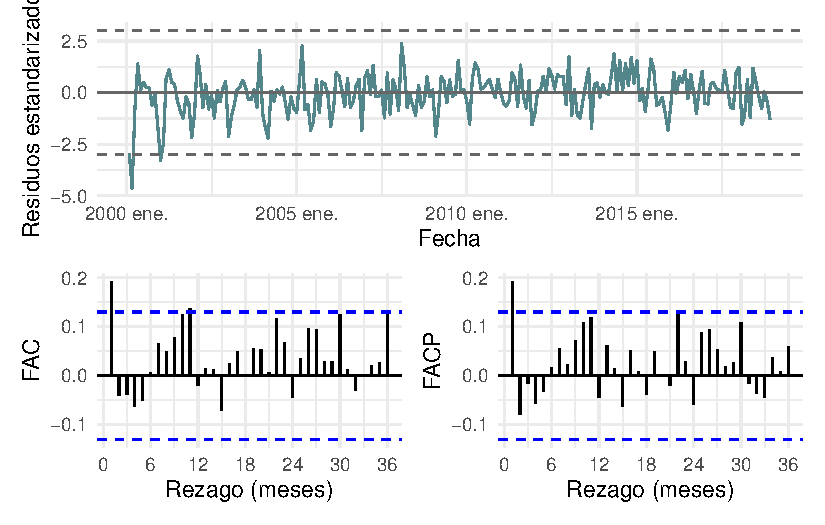
\includegraphics[keepaspectratio]{TP-MInesCañizares_files/figure-pdf/fig-res-m1-1.pdf}}

}

\caption{\label{fig-res-m1}Residuos estandarizados del modelo
ARIMA(0,1,1)(0,1,1){[}12{]}, con su FAC y FACP}

\end{figure}%

Los residuos estandarizados oscilan alrededor de cero con variabilidad
aproximadamente constante, aunque se observan dos valores por fuera del
intervalo \((-3, 3)\) al inicio de la serie. En la FAC y la FACP el
rezago 1 supera claramente la banda de significancia, y los rezagos 10 y
11 se ubican en el límite. Esto es coherente con el resultado del test
de Portmanteau: persiste dependencia de corto plazo no capturada por el
modelo.

\begin{figure}

\centering{

\pandocbounded{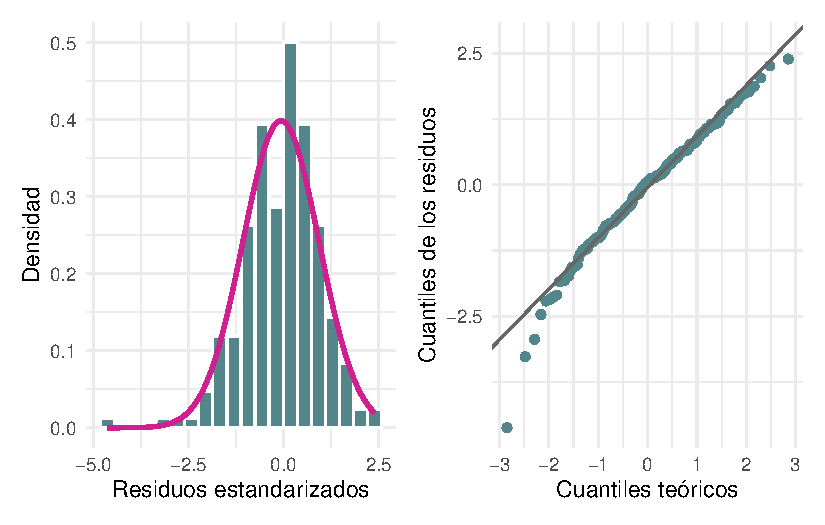
\includegraphics[keepaspectratio]{TP-MInesCañizares_files/figure-pdf/fig-norm-m1-1.pdf}}

}

\caption{\label{fig-norm-m1}Histograma y QQ-plot de los residuos
estandarizados del modelo ARIMA(0,1,1)(0,1,1){[}12{]}}

\end{figure}%

El histograma se aproxima a una distribución normal, con una cola
izquierda algo más pesada. En el QQ-plot los puntos siguen la recta,
salvo en el extremo inferior, donde se separan los valores atípicos
mencionados. Además, se realizó el test de Shapiro-Wilk sobre los
residuos para evaluar normalidad, el cuál rechazamla hipótesis (p-value
= 0,0010). Este apartamiento se concentra en la cola izquierda y se debe
a las observaciones atípicas del inicio de la serie.

En síntesis, aunque los coeficientes son significativos, este modelo no
pasa el diagnóstico: los residuos presentan autocorrelación remanente y
no son normales.

Se procede a comparar ambos modelos considerados:

{

\begin{longtable}[]{@{}cccc@{}}

\caption{\label{tbl-comparacion}Comparación de los modelos SARIMA
considerados}

\tabularnewline

\toprule\noalign{}
Modelo & AICc & BIC & MAPE (\%) \\
\midrule\noalign{}
\endhead
\bottomrule\noalign{}
\endlastfoot
ARIMA(0,1,1)(0,1,1){[}12{]} & -4870.79 & -4860.62 & 3.61 \\
ARIMA(0,1,2)(0,1,1){[}12{]} & -4874.32 & -4860.80 & 3.57 \\

\end{longtable}

}

En síntesis, el modelo \(\text{SARIMA}(0,1,2)(0,1,1)_{12}\) presenta
coeficientes significativos y residuos sin autocorrelación remanente,
con la salvedad de la falta de normalidad debida a dos observaciones
atípicas.

Al comparar ambos modelos (Tabla Tabla~\ref{tbl-comparacion}), el
\(\text{SARIMA}(0,1,2)(0,1,1)_{12}\) presenta un AICc menor (diferencia
de aproximadamente 3,5 puntos), mientras que el BIC y el MAPE son
prácticamente equivalentes. Dado que los criterios de información no
distinguen claramente entre ambos, el diagnóstico de los residuos
resulta determinante: el \(\text{SARIMA}(0,1,2)(0,1,1)_{12}\) es el
único cuyos residuos no muestran autocorrelación remanente, y todos sus
coeficientes son significativos. Por lo tanto, se lo selecciona como
modelo final para la etapa de pronóstico.

\section{Evaluación predictiva del modelo
seleccionado}\label{evaluaciuxf3n-predictiva-del-modelo-seleccionado}

Para la etapa de pronósticos, se ajusta el modelo SARIMA seleccionado
utilizando los datos disponibles hasta diciembre de 2018 y se generan
predicciones para las doce observaciones del año 2019, que constituyen
la muestra de evaluación. Además, se comparan los valores pronosticados
con los datos reales de 2019 a fin de evaluar el desempeño del modelo y
analizar su capacidad predictiva.

{\def\LTcaptype{none} % do not increment counter
\begin{longtable}[]{@{}cccc@{}}
\toprule\noalign{}
Mes & Valor real & Pronóstico & IC del 95\% \\
\midrule\noalign{}
\endhead
\bottomrule\noalign{}
\endlastfoot
enero & 13.447 & NA & (NA; 3434) \\
febrero & 12.125 & NA & (NA; 2985) \\
marzo & 13.433 & NA & (NA; 2909) \\
abril & 12.443 & NA & (NA; 2743) \\
mayo & 12.232 & NA & (NA; 2637) \\
junio & 11.556 & NA & (NA; 2508) \\
julio & 11.870 & NA & (NA; 2444) \\
agosto & 11.816 & NA & (NA; 2378) \\
septiembre & 11.752 & NA & (NA; 2303) \\
octubre & 12.693 & NA & (NA; 2285) \\
noviembre & 12.955 & NA & (NA; 2236) \\
diciembre & 13.683 & NA & (NA; 2217) \\
\end{longtable}
}




\end{document}
